\documentclass[border=3pt]{standalone}
\usepackage{tikz}
\usetikzlibrary{arrows.meta,calc}
\begin{document}
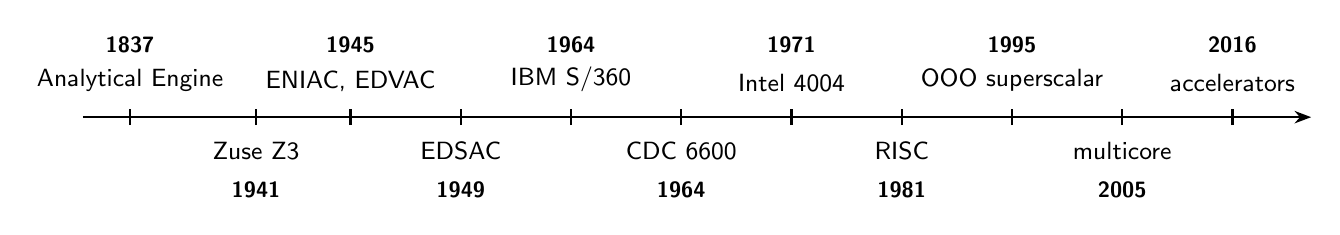
\begin{tikzpicture}[font=\sffamily\small]
  % axis
  \draw[thick,-{Stealth[length=6pt]}] (0,0) -- (15.6,0);
  % ticks: x, year, label above/below
  \foreach \x/\yr/\pos/\lbl in {
    0.6/1837/above/{Analytical Engine},
    2.2/1941/below/{Zuse Z3},
    3.4/1945/above/{ENIAC, EDVAC report},
    4.8/1949/below/{EDSAC (stored program)},
    6.2/1964/above/{IBM System/360},
    7.6/1964/below/{CDC 6600},
    9.0/1971/above/{Intel 4004},
    10.4/1981/below/{RISC (801, MIPS)},
    11.8/1995/above/{OOO superscalar},
    13.2/2005/below/{multicore era},
    14.6/2016/above/{accelerators}}{
    \draw[thick] (\x,-0.1) -- (\x,0.1);
    \ifx\pos\relax\else\fi
  }
  \foreach \x/\yr/\lbl in {0.6/1837/{Analytical Engine},3.4/1945/{ENIAC, EDVAC},6.2/1964/{IBM S/360},9.0/1971/{Intel 4004},11.8/1995/{OOO superscalar},14.6/2016/{accelerators}}{
    \node[above=1mm] at (\x,0.1) {\lbl};
    \node[above=6mm, font=\sffamily\footnotesize\bfseries] at (\x,0.1) {\yr};
  }
  \foreach \x/\yr/\lbl in {2.2/1941/{Zuse Z3},4.8/1949/{EDSAC},7.6/1964/{CDC 6600},10.4/1981/{RISC},13.2/2005/{multicore}}{
    \node[below=1mm] at (\x,-0.1) {\lbl};
    \node[below=6mm, font=\sffamily\footnotesize\bfseries] at (\x,-0.1) {\yr};
  }
\end{tikzpicture}
\end{document}
